%!TEX root = main.tex

\chapter{Results}
This chapter presents results of how our implementation performed.

\section{Agent performance}
In this section we describe the performance test we ran and the results that it yielded.
\subsection{The test}
To measure how well the agent performed when it played  we ran 50 games against the built-in AI in StarCraft Brood War. We only ran 50 games because the performance of the agent is very dependent on how how many feature detectors are implemented and how much of the game that the agent is capable of understanding. Because we only implemented a very basic agent as proof of concept it will not be smart enough to handle all the situations that it will get into, and therefor the performance is not any good measurement of how well the method will perform if expanded upon with more complex detectors and schemes. 
	
All the games where played on the same map, Astral Balance, to avoid any map specific problems that could mess with the agents performance. As explained in section \ref{sec:overview} our agent only played as the Protoss race, and the enemy was set to random so they could be any of the three available races. We gave the agent access to perfect information in the game, because the built-in AI also utilizes perfect information, and that means it does not have to scout to know where the enemy is located.

\subsection{The result}
Table \ref{tab:test_results} shows the results from the performance test. After the 50 games we ended up with 17 victories and 33 defeats. Something that equals a win percentage of 34\%. In a few situations the agent got stuck after it had destroyed all the enemy buildings and unit except for one or two in an expansion or hiding in a corner. These games we judged as a win because the enemy had no chance of rebuilding no matter how long it was left alone in this state.

\begin{table}
\begin{center}
\begin{tabular}{| c | c |}
  \hline                        
  Victories & Defeats\\
  \hline
  17 & 33 \\
  \hline  
\end{tabular}
\caption{Results from performance test}
\label{tab:test_results}
\end{center}
\end{table}

\section{A cognitive cycle}
A cognitive cycle is the a sequence of processes that the cognitive model has to go through from sensing to execution of an action. In LIDA the sequence starts with sensing of the environment, next is understanding, then attention and last is the selection of an action and its execution. These cycles run constantly, and even several of them runs at the same time just in different stages. So when one cycle is finishing broadcasting from the global workspace another can be starting in the sensing phase. 

Following we describe the complete cognitive cycle that ends with the creation of a new worker unit. 	

\subsection{Sensing}
The first step in the cognitive cycle is sensing. Here sensory-memory samples the environment for new input to the model before low level feature detectors analyzes the input looking for specific features, ideas and meanings. If the feature detector finds something it sends excitation to a corresponding feature node in the perceptual associative memory(PAM). The amount of excitation can be anything from zero to one, depending on how important or present the given feature is currently. Figure \ref{fig:pamtable} shows the table of nodes that we implemented in the project, this is before Starcraft starts running so all the nodes have zero activation yet.See section \ref{sec:detectors} for a list of what detectors we implemented in our agent that will feed activation to these nodes. 

\begin{figure}[h!tb]
\centering
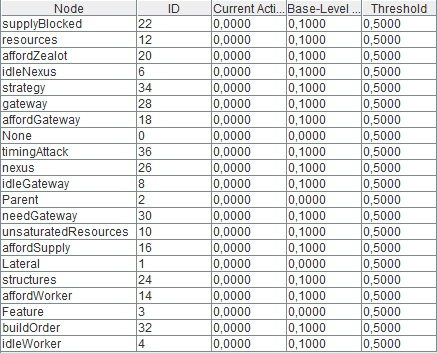
\includegraphics[scale=1.0]{graphics/pam_table.png}
\caption{The PAM table with current activation values}
\label{fig:pamtable}
\end{figure}

When a node receives excitation it also sends a portion of this excitation upstream to any node that it has as a parent. This way meta nodes like {\em resources} and {\em structures} can receive activation even though there are no feature detectors that directly affects this node. Figure \ref{fig:pamgraph} shows our current PAM graph with the relationships  between the nodes. 

\begin{figure}[h!tb]
\centering
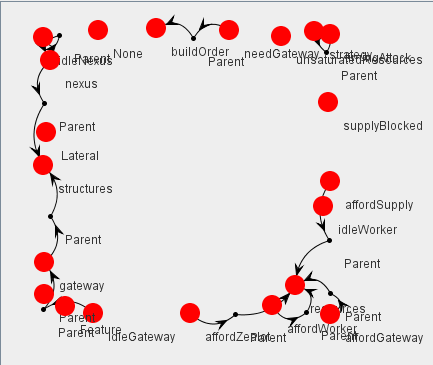
\includegraphics[scale=1.0]{graphics/pam_graph.png}
\caption{Representation of the PAM graph}
\label{fig:pamgraph}
\end{figure}


\subsection{Understanding}
After the sensing phase and nodes in PAM have received excitation, any node that has an activation that is higher then the threshold will be moved to the Perceptual Buffer that is a sub module of the Workspace module. Te content of this buffer and any relevant information from the Transient Episodic Memory and Declarative Memory will make up the Current Situational Model. The CSM has the structures that represents the agents current understanding of the world. Since we do not utilize the TEM and DM modules CSM contains only data from the Perceptual Buffer. Figure \ref{fig:csm} shows the content of CSM for our current cycle. 

\begin{figure}[h!tb]
\centering
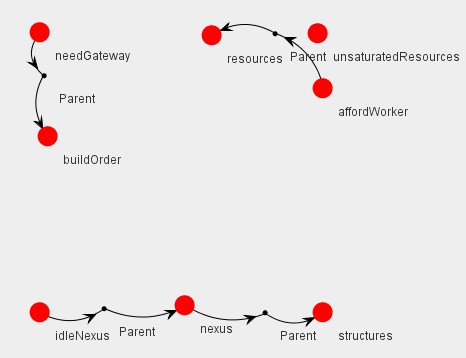
\includegraphics[scale=1.0]{graphics/perceptual_buffer.png}
\caption{The node structure in the CSM}
\label{fig:csm}
\end{figure}

We can see that the agent knows that we can afford to make a worker and that our resources, our mineral line, is not saturated. It also knows that the nexus is idle, not producing any units at the moment. These are the relevant pieces of information for creating a worker. But the CSM also contains information about the need for a gateway, but because we can't afford it it will not be selected as a focus for consciousness in the next phase.


\subsection{Attention}
After the CSM is updated the competition for consciousness begins. It is the job of attention codelets to bring important or urgent content to consciousness. The attention codelet creates a coalition of content from the CSM and gains activation based on the activation of both the nodes it gathers and the activation level of the codelet itself. All the codelets that are active, can be both new codelets and codelets from a previous cycles that has not yet decayed, then compete for the chance to be broadcast from the global workspace. In figure \ref{fig:workspace} we can see the codelets competing for consciousness in this cycle. We can see that the codelet with a coalition of idleNexus, unsaturatedResources and affordWorker has the highest activated and will win the competition. It will therefor be the focus of consciousness when it is broadcast from the Global Workspace. 

\begin{figure}[h!tb]
\centering
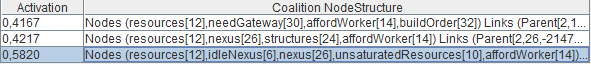
\includegraphics[width=\textwidth]{graphics/global_workspace.png}
\caption{Content of the global workspace}
\label{fig:workspace}
\end{figure}

The coalition that gets broadcast is used for learning in several of the LIDA modules. But because learning is not implemented in the current version of the LIDA framework we could not utilize this. 

\subsection{Action selection}
\label{sec:action_selection}
The last phase of the LIDA cognitive cycle is the action selection. The first step of this phase is the Procedural Memory receiving the conscious broadcast from the Global Workspace. The Procedural Memory contains the scheme net and using the information from the broadcast some of the schemes will increase their activation if their context is contained in the broadcast. The schemes are put above their threshold are instantiated as behaviors and then sent to the Action Selection module. Figure \ref{fig:proceduralmemory} shows all the available schemes in our implementation, and the current activated scheme is the one with the action to create a worker. The build worker scheme is activated because all of the nodes in its context was received with the conscious broadcast from last phase. 

\begin{figure}[h!tb]
\centering
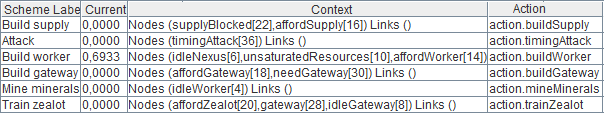
\includegraphics[width=\textwidth]{graphics/procedural_memory.png}
\caption{Content of the procedural memory}
\label{fig:proceduralmemory}
\end{figure}

After some schemes are activated into behaviors they are received by the Action Selection module, where the final decision about what action is going to be performed in this cycle taken. The LIDA module describes this module as a behavior network\cite{maes1989right}. But in the current version of the LIDA framework this has not been implemented yet. So in the current version the Action Selection module is very simplified. And that makes it harder to do complex selections. The current action selection mainly just selects the behavior with the highest activation. So the real selection actually happens in the Procedural Memory. But with the release of the next version of the framework that should change(May 2012). Figure \ref{fig:actionselection} shows the content of the Action Selection module for this cognitive cycle. Our one behavior doesn't have any competition so it is selected as the action to perform this cycle. And below are a list of the five last performed actions in past cycles. 
\begin{figure}[h!tb]
\centering
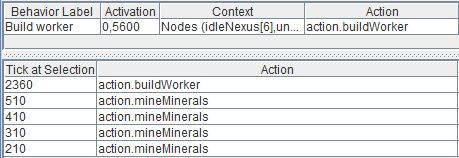
\includegraphics[scale=1.0]{graphics/action_selection.png}
\caption{Content of the action selection module}
\label{fig:actionselection}
\end{figure}

When the action is selected it is passed on to the Sensory-Motor Memory that will use its actuators on the environment to execute the action. In our cycle this will involve starting to build a worker unit from the Nexus building. 